\subsection{Phonotactic Language Models}
\label{sec:phonotactic}

Estimation of a probabilistic transcription from mismatched
crowdsourcing is improved if we have information about phone sequences
in the spoken language. By assumption, such information is not
available from speech: we assume that there is no transcribed speech
in the target language.  A reasonable proxy, however, can be
constructed from text.

\begin{figure}
  \centerline{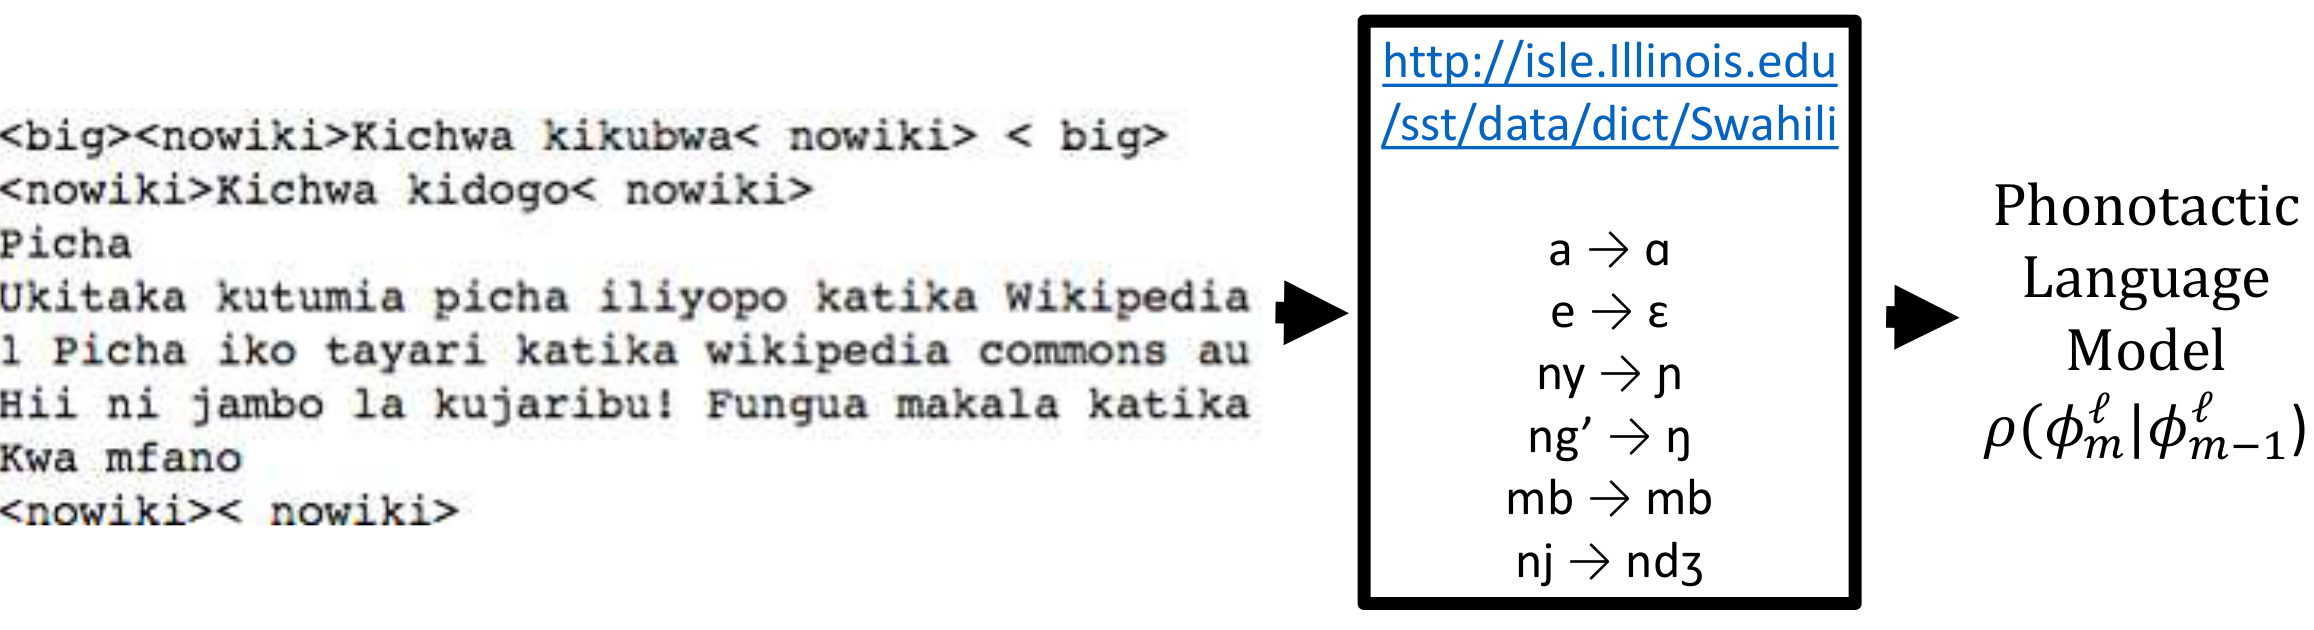
\includegraphics[width=5in]{../figs/fig_sloan.png}}
  \caption{A phonotactic language model (a bigram language model over
    phone sequences) can be trained using text data downloaded from
    Wikipedia (left), then converted into phone strings in the target
    language using a simple character-based grapheme-to-phoneme
    transducer (center).  In this example, the target language is
    Swahili.}
  \label{fig:wikitext}
\end{figure}

Fig.~\ref{fig:wikitext} shows text data downloaded from Wikipedia in
Swahili, and a segment of a rule-based, character-by-character G2P for
the Swahili language~\cite{Hasegawajohnson15}.  By passing the former
through the latter, it is possible to generate synthetic phoneme
sequences in the target language.

\begin{figure}
  \centerline{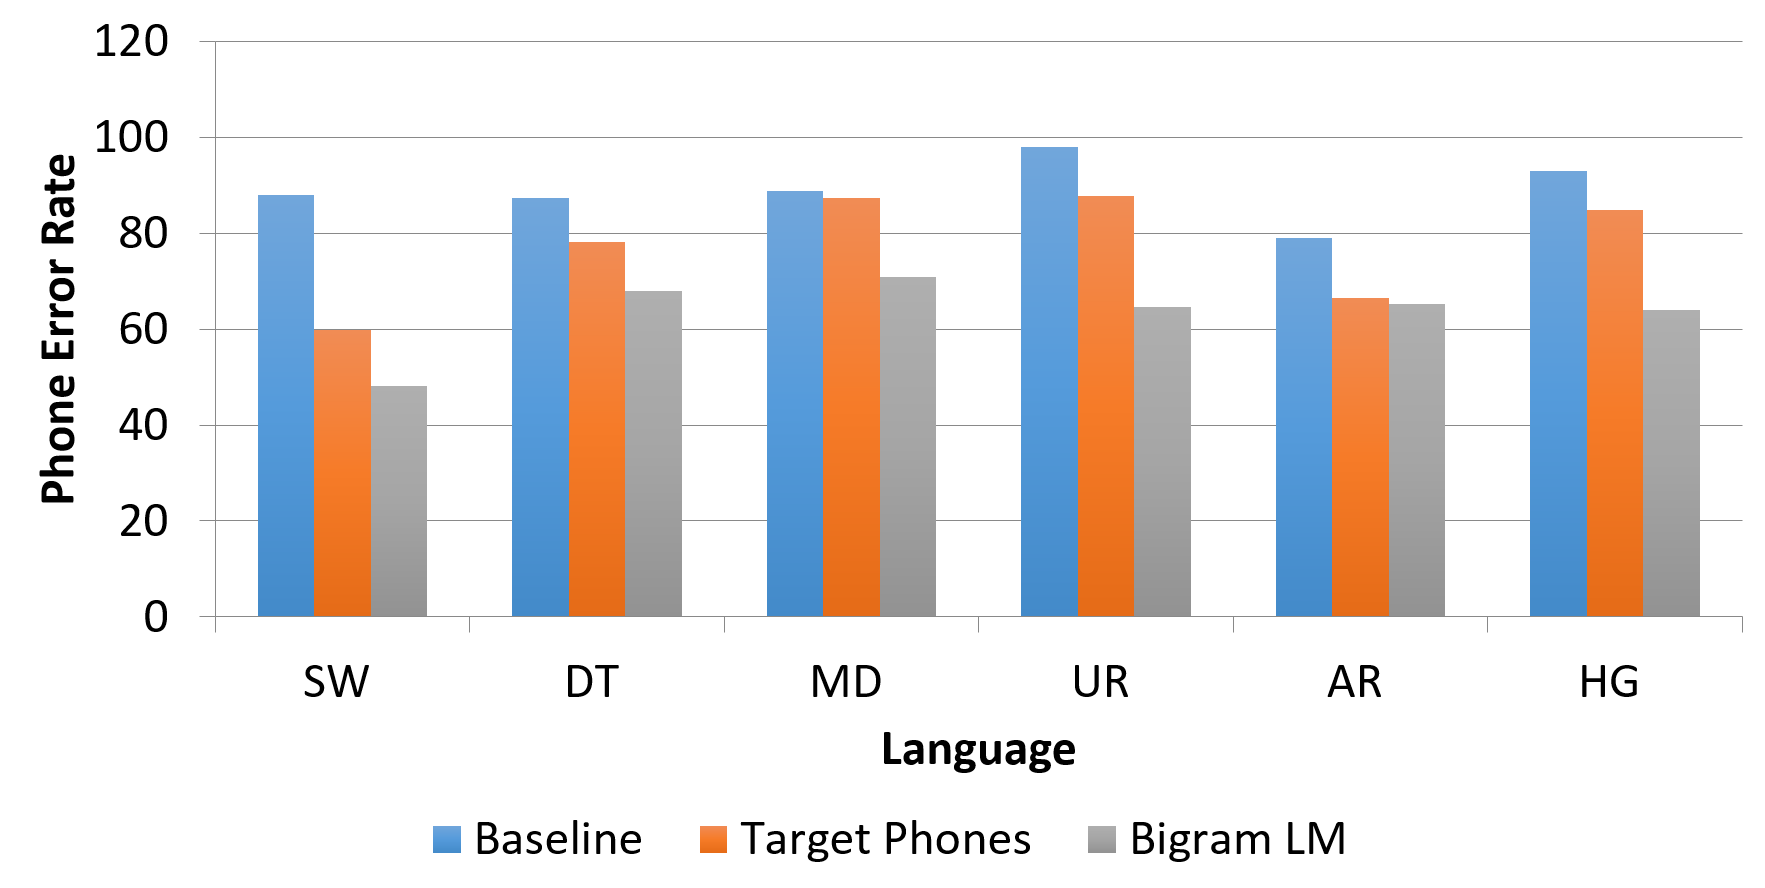
\includegraphics[width=4in]{../figs/sloan2.png}}
  \caption{PER of the 1-best path: a measure of the quality of
    probabilistic transcriptions acquired from mismatched
    crowdsourcing.  Native transcriptions were available in six
    languages: Swahili (SW), Dutch (DT), Mandarin (MN), Urdu (UR),
    Arabic (AR), and Hungarian (HG).  Probabilistic transcriptions
    were decoded using three different methods per language: using a
    universal phoneme set (tallest bar in each language), using a
    phoneme set specific to the target language (middle bar in each
    language), and using a phonotactic language model derived from
    Wikipedia texts (shortest bar in each language).}
  \label{fig:pt_decode_per}
\end{figure}

Phone error rate of the 1-best path through the mismatched
crwodsourcing confusion network are shown in
Fig.~\ref{fig:pt_decode_per}.  As shown, the use of a phonotactic
language model, derived from Wikipedia text, reduced phone error rate
by about 10\% absolute, in each language.

